\documentclass[tikz,border=5pt]{standalone}
\pdfinfoomitdate=1
\pdftrailerid{}
\pdfsuppressptexinfo=-1
\usepackage{pgfplots}
\usepgfplotslibrary{groupplots}
\pgfplotsset{compat=1.18}
\pgfplotsset{colormap/viridis}
\definecolor{atlas0}{HTML}{0072B2}
\definecolor{atlas1}{HTML}{D55E00}
\definecolor{atlas2}{HTML}{009E73}
\definecolor{atlas3}{HTML}{E69F00}
\definecolor{atlas4}{HTML}{56B4E9}
\definecolor{atlas5}{HTML}{CC79A7}
\definecolor{atlas6}{HTML}{000000}
\definecolor{atlas7}{HTML}{F0E442}
% NATO SERS figure F42; data_sha256=9b814b0234b849393cbd192f71d73b56e0554964a4e14d851044bdd40d4b2ce1
% caption=(S) RQ-P01 C09 reliability after scalar temperature calibration fitted only to source-development cross-fitted scores. Ten fixed-width confidence bins are computed per technical repeat, then bin confidence and accuracy are averaged across repeats; vertical intervals are the observed repeat range, not confidence intervals. The diagonal is perfect calibration. Only endpoints with valid calibrated probabilities enter; omissions remain in endpoint coverage. PP-U-MIN and no held-target calibration statistics.
\begin{document}
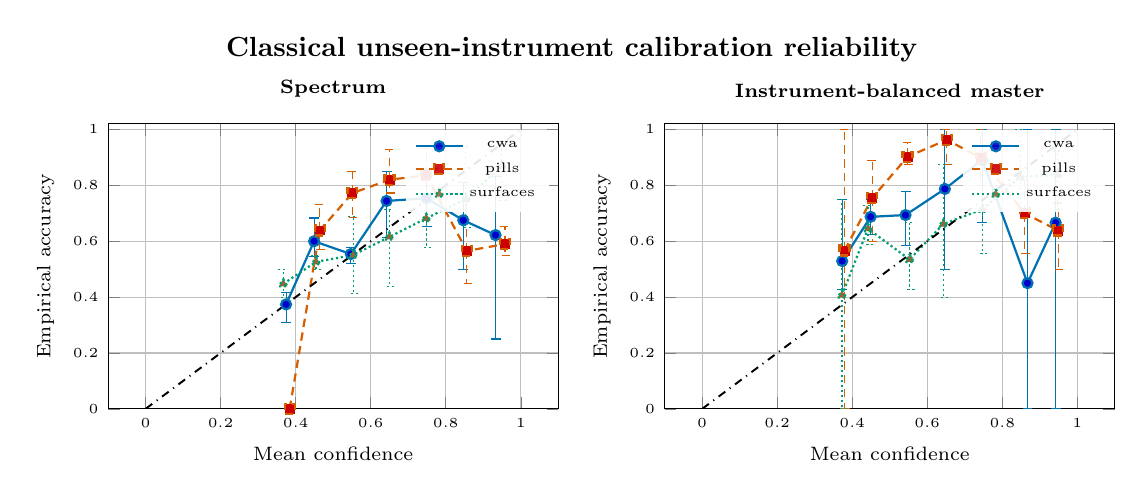
\begin{tikzpicture}
\begin{groupplot}[group style={group size=2 by 1, horizontal sep=1.35cm, vertical sep=1.5cm}, width=7.30cm, height=5.2cm, grid=major, tick label style={font=\tiny}, label style={font=\scriptsize}, title style={font=\scriptsize\bfseries,align=center}, legend style={font=\tiny,draw=none,fill=white,fill opacity=0.9,text opacity=1}]
\nextgroupplot[title={Spectrum},xlabel={Mean confidence},ylabel={Empirical accuracy},ymin=0,ymax=1.02]
\addplot+[color=atlas0,mark=*,mark size=1.8pt,line width=0.8pt,solid,error bars/.cd,y dir=both,y explicit] coordinates {(0.37434515,0.3739891) += (0,0.042677566) -= (0,0.066296793) (0.44902867,0.60007921) += (0,0.083254123) -= (0,0.054624665) (0.54701342,0.55410684) += (0,0.022816239) -= (0,0.034106838) (0.64217434,0.74421352) += (0,0.10578648) -= (0,0.1313103) (0.74870232,0.75417216) += (0,0.079161177) -= (0,0.10199824) (0.84669369,0.6752381) += (0,0.13428571) -= (0,0.1752381) (0.93269813,0.62212121) += (0,0.21121212) -= (0,0.37212121)};
\addlegendentry{cwa}
\addplot+[color=atlas1,mark=square*,mark size=1.8pt,line width=0.8pt,densely dashed,error bars/.cd,y dir=both,y explicit] coordinates {(0.38394788,0) += (0,0) -= (0,0) (0.46421759,0.63850329) += (0,0.092265945) -= (0,0.067074715) (0.5511747,0.77233487) += (0,0.076149978) -= (0,0.088124344) (0.65016852,0.82033703) += (0,0.10823439) -= (0,0.047609762) (0.74837057,0.83613894) += (0,0.09719439) -= (0,0.071433061) (0.85614503,0.56533696) += (0,0.17659853) -= (0,0.11706109) (0.95787094,0.59007172) += (0,0.062102198) -= (0,0.040775941)};
\addlegendentry{pills}
\addplot+[color=atlas2,mark=triangle*,mark size=1.8pt,line width=0.8pt,densely dotted,error bars/.cd,y dir=both,y explicit] coordinates {(0.36677828,0.44733193) += (0,0.052668067) -= (0,0.047331933) (0.45418083,0.52624289) += (0,0.023757111) -= (0,0.026242889) (0.55301867,0.55042765) += (0,0.13707235) -= (0,0.13866295) (0.6491889,0.61534178) += (0,0.098943932) -= (0,0.17784178) (0.7475607,0.68167641) += (0,0.068323587) -= (0,0.10272904) (0.85375208,0.75177132) += (0,0.18940515) -= (0,0.10177132) (0.94893265,0.86888023) += (0,0.092658235) -= (0,0.12419938)};
\addlegendentry{surfaces}
\addplot[black,dashdotted,line width=0.7pt,forget plot] coordinates {(0,0) (1,1)};
\nextgroupplot[title={Instrument-balanced master},xlabel={Mean confidence},ylabel={Empirical accuracy},ymin=0,ymax=1.02]
\addplot+[color=atlas0,mark=*,mark size=1.8pt,line width=0.8pt,solid,error bars/.cd,y dir=both,y explicit] coordinates {(0.37317165,0.52912088) += (0,0.22087912) -= (0,0.10054945) (0.44905921,0.68746377) += (0,0.062536232) -= (0,0.062463768) (0.54196882,0.69386724) += (0,0.083910534) -= (0,0.11053391) (0.64679377,0.78727273) += (0,0.21272727) -= (0,0.28727273) (0.74640871,0.89166667) += (0,0.10833333) -= (0,0.225) (0.86706953,0.45) += (0,0.55) -= (0,0.45) (0.9419842,0.66666667) += (0,0.33333333) -= (0,0.66666667)};
\addlegendentry{cwa}
\addplot+[color=atlas1,mark=square*,mark size=1.8pt,line width=0.8pt,densely dashed,error bars/.cd,y dir=both,y explicit] coordinates {(0.37943595,0.56666667) += (0,0.43333333) -= (0,0.56666667) (0.45314205,0.75502415) += (0,0.13386473) -= (0,0.15502415) (0.54741011,0.9025873) += (0,0.049793651) -= (0,0.027587302) (0.65234037,0.96323529) += (0,0.036764706) -= (0,0.088235294) (0.74247991,0.89794872) += (0,0.10205128) -= (0,0.097948718) (0.85929381,0.70005112) += (0,0.1181307) -= (0,0.14449556) (0.94916514,0.63834881) += (0,0.098493292) -= (0,0.13834881)};
\addlegendentry{pills}
\addplot+[color=atlas2,mark=triangle*,mark size=1.8pt,line width=0.8pt,densely dotted,error bars/.cd,y dir=both,y explicit] coordinates {(0.37256466,0.40714286) += (0,0.34285714) -= (0,0.40714286) (0.44186726,0.64500637) += (0,0.082266361) -= (0,0.056771072) (0.55286609,0.53480519) += (0,0.13186147) -= (0,0.10623377) (0.64236404,0.66127451) += (0,0.21372549) -= (0,0.26127451) (0.74713642,0.71444444) += (0,0.28555556) -= (0,0.15888889) (0.84739062,0.83095238) += (0,0.16904762) -= (0,0.11666667) (0.94768157,0.83757354) += (0,0.085503386) -= (0,0.12328782)};
\addlegendentry{surfaces}
\addplot[black,dashdotted,line width=0.7pt,forget plot] coordinates {(0,0) (1,1)};
\end{groupplot}
\node[font=\normalsize\bfseries,anchor=south] at (current bounding box.north) {Classical unseen-instrument calibration reliability};
\end{tikzpicture}
\end{document}
